% Niveau :      PCSI - PC
% Discipline :  Méca
% Mots clés :   Hohmann

\begin{exercise}{Orbite de Hohmann}{2}{Sup,Spé}
{Mécanique,Mécanique céleste}{lelay}

On cherche à mettre un satellite en orbite géostationnaire. Dans un premier temps, on le met en orbite circulaire autour de la Terre à une altitude de 300 km au dessus du sol.

\begin{questions}
    \questioncours Donner l'expression et la valeur altitude d'un satellite géostationnaire.
    \question Donner l'énergie mécanique d'un satellite en orbite stationnaire à un rayon $R$ autour de la Terre en fonction de $R$ et d'une constante $K$ que l'on précisera. En déduire par analogie l'énergie de ce satellite sur une orbite elliptique de demi grand axe $a$.
    \question En repartant de la formule générale de l'énergie mécanique, donner la vitesse $v$ d'un mobile de masse $m$ en orbite elliptique autour de la Terre en fonction de $r$, $a$ et de $K$.
    \question On veut passer d'une orbite circulaire de rayon $R_-$ à une orbite circulaire de rayon $R_+$ en utilisant une \textit{orbite de transfert} elliptique, de manière à utiliser le moins de carburant possible (minimiser les phases d'accélération). Faire un schéma et proposer une telle orbite.
    \question Donner la quantité totale d'énergie cinétique à fournir en tout. Montrer qu'elle est minimale.
    \question Expliquer pourquoi cette technique est utilisée pour les voyages visant à rejoindre l'ISS.
\end{questions}
\end{exercise}

\begin{solution}

\begin{questions}
    \questioncours 3e loi de Kepler $R^3/T^2 = GM/4\pi^2$ d'où avec $T = $24 h, $R = 42300$ km, d'où une \textbf{altitude} d'environ 36000 km.
    \question On a (3e loi de Kepler) $R^3\omega^2 = GM$ or $v = R\omega$ soit $v = \sqrt{GM/R} = \sqrt{K/R}$ avec $K = GM$. D'où l'énergie mécanique $E = \frac12 m v^2 - \frac{mMG}{R} = \frac12 \frac{Km}{R} - \frac{Km}{R} = -\frac12\frac{Km}{R}$ on retrouve le résultat bien connu. On généralise pour une ellipse en remplaçant $R$ par $a$ : $E = -\frac12\frac{Km}{a}$
    \question On a $E = \frac12m v^2 - \frac{Km}{r}$ soit $v^2 = -\frac{K}{a} - \qty(-\frac{K}{2r})$ d'où $v = \sqrt{K}\sqrt{\frac2r-\frac1a}$
    \question Il faut en gros proposer le schéma suivant :
    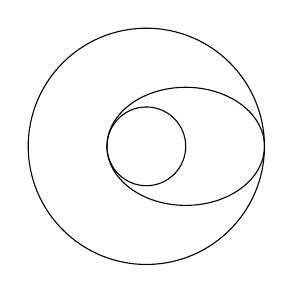
\begin{tikzpicture}
    
    \draw (0,0) ellipse (0.5);
    \draw (0.5,0) ellipse (1 and 0.75);
    \draw (0,0) ellipse (1.5);
    
    \end{tikzpicture}
    La petite orbite est l'orbite initiale, la grande l'orbite finale, et entre les deux une orbite qui interpole.
    Il y a donc 3 étapes, et pour passer de chaque orbite a la suivante on met un coup d'accélérateur, i.e. on change de vitesse.
    Le demi grand axe de l'orbite de Hohmann est évidemment $a = (R_- + R_+)/2$.
    \question 
    \begin{itemize}
        \item Transition départ -> Hohmann : la vitesse passe de $v = \sqrt{\frac{K}{R_-}}$ à $v' = \sqrt{K}\sqrt{\frac{2}{R_-}-\frac1a}$ d'où $\Delta {E_c}_1 = \frac1{2} m ({v'}^2 - v^2) = \frac{12}mK\qty(\frac{1}{R_-} - \frac1a)$
        \item Transition Hohmann -> arrivée : la vitesse passe de $v = \sqrt{K}\sqrt{\frac{2}{R_+}-\frac1a}$ à $v' = \sqrt{\frac{K}{R_+}}$ d'où $\Delta {E_c}_2 = \frac1{2} m ({v'}^2 - v^2) = \frac{12}mK\qty(\frac{1}{a} - \frac1{R_+})$
    \end{itemize}
    Au total on a donc dépensé une énergie $\Delta {E_c}_1 + \Delta {E_c}_2 = \frac{12}mK\qty(\frac{1}{R_-} - \frac1{R_+}) = {E_m}_\text{finale} - {E_m}_\text{initiale}$ : aucune dépense superflue.
    \question C'est la moins coûteuse en énergie puisqu'elle est optimale. En pratique on utilise plusieurs orbites de transfert, en diminuant l'ellipticité quand on s'approche de la cible (3 orbites pour l'ISS).
\end{questions}

Masse de la Terre : $6\cdot 10^{24}$ kg

Rayon de la Terre : 6400 km
\end{solution}